\documentclass[border=12pt]{standalone}
\usepackage{tikz}
\usetikzlibrary{shapes.geometric, arrows.meta, positioning, calc, fit, backgrounds}
\usepackage{fontspec}
\usepackage{amsmath,amssymb}
\setmainfont{DejaVu Sans}

\begin{document}
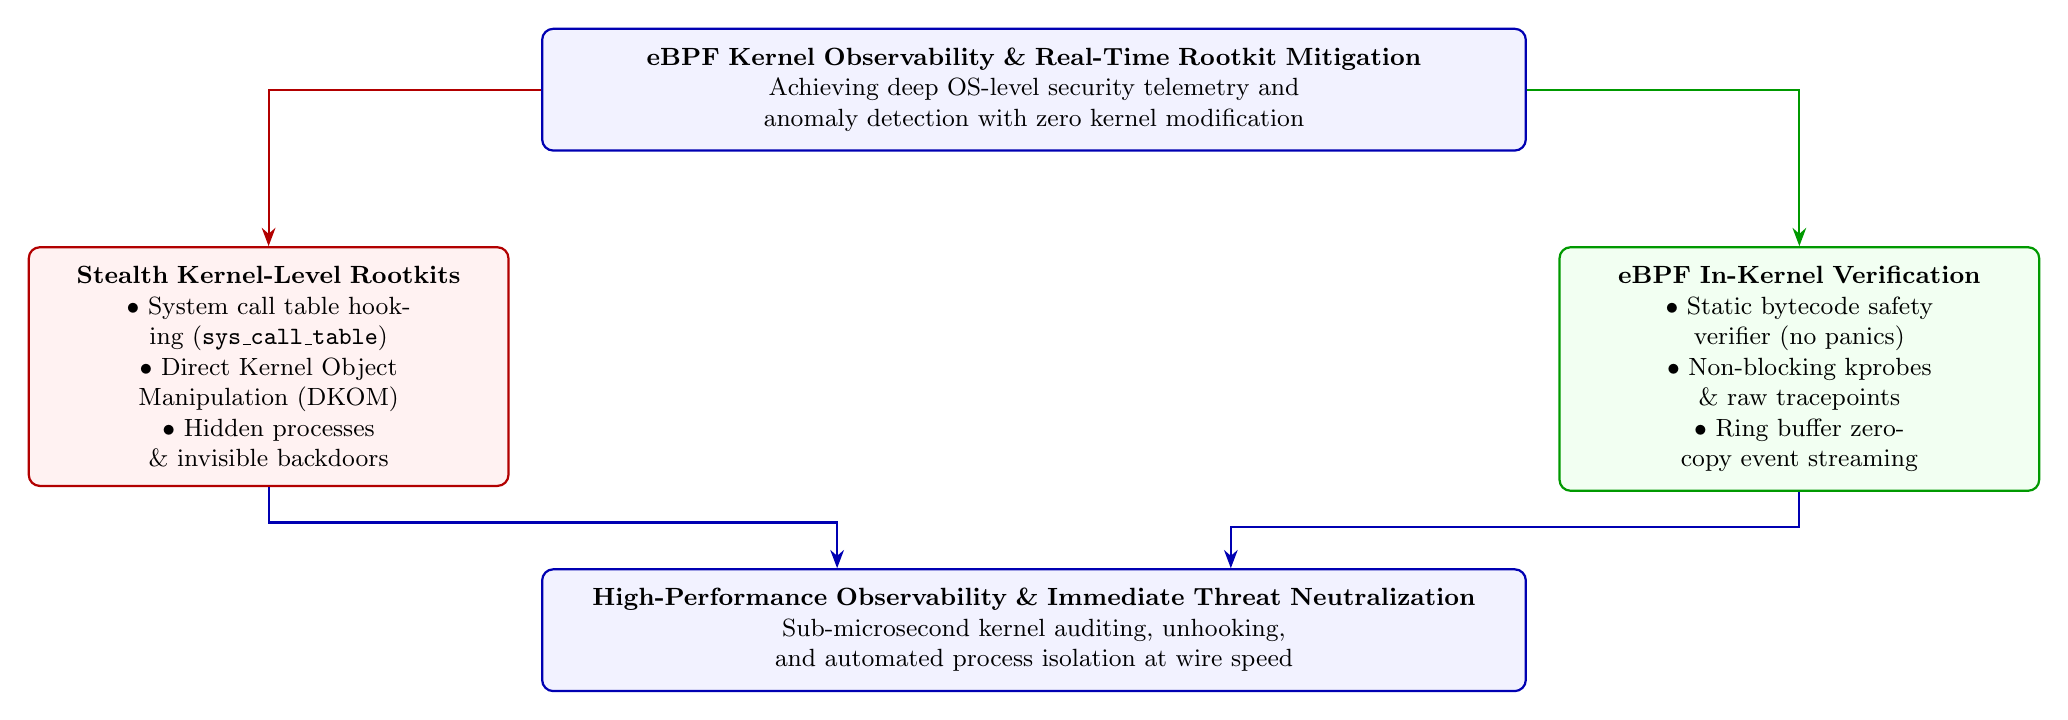
\begin{tikzpicture}[
    font=\small,
    >=Stealth,
    node distance=1.2cm,
    block/.style={rectangle, draw=blue!70!black, fill=blue!5, rounded corners=4pt, thick, align=center, inner sep=7pt},
    alertblock/.style={rectangle, draw=red!70!black, fill=red!5, rounded corners=4pt, thick, align=center, inner sep=7pt},
    greenblock/.style={rectangle, draw=green!60!black, fill=green!5, rounded corners=4pt, thick, align=center, inner sep=7pt},
    amberblock/.style={rectangle, draw=orange!80!black, fill=orange!5, rounded corners=4pt, thick, align=center, inner sep=7pt}
]

\node[block, text width=12cm] (top) {\textbf{eBPF Kernel Observability \& Real-Time Rootkit Mitigation}\\Achieving deep OS-level security telemetry and anomaly detection with zero kernel modification};

\node[alertblock, below left=1.2cm and 0.4cm of top, text width=5.6cm] (rootkit_threat) {\textbf{Stealth Kernel-Level Rootkits}\\$\bullet$ System call table hooking (\texttt{sys\_call\_table})\\$\bullet$ Direct Kernel Object Manipulation (DKOM)\\$\bullet$ Hidden processes \& invisible backdoors};

\node[greenblock, below right=1.2cm and 0.4cm of top, text width=5.6cm] (ebpf_engine) {\textbf{eBPF In-Kernel Verification}\\$\bullet$ Static bytecode safety verifier (no panics)\\$\bullet$ Non-blocking kprobes \& raw tracepoints\\$\bullet$ Ring buffer zero-copy event streaming};

\node[block, below=1.0cm of $(rootkit_threat.south)!0.5!(ebpf_engine.south)$, text width=12cm] (bottom) {\textbf{High-Performance Observability \& Immediate Threat Neutralization}\\Sub-microsecond kernel auditing, unhooking, and automated process isolation at wire speed};

\draw[->, thick, red!70!black] (top) -| (rootkit_threat);
\draw[->, thick, green!60!black] (top) -| (ebpf_engine);
\draw[->, thick, blue!70!black] (rootkit_threat.south) -- ++(0,-0.45) -| ([xshift=-2.5cm]bottom.north);
\draw[->, thick, blue!70!black] (ebpf_engine.south) -- ++(0,-0.45) -| ([xshift=2.5cm]bottom.north);

\end{tikzpicture}
\end{document}
